\vspace{-3pt}
\section{The Muon Detector System}\label{sec:ch3:muon}

\begin{figure}[h]
\centering
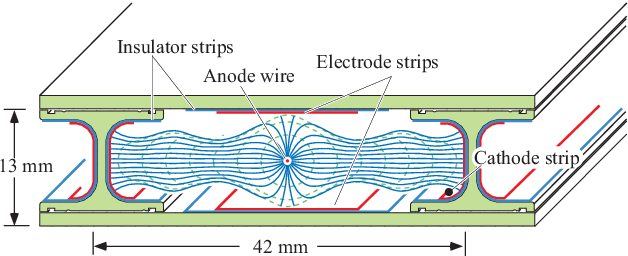
\includegraphics[width=0.75\textwidth]{figures/muon_DT_schematic.png}
\caption{Schematic of a muon detector drift tube~\cite{drift_tube_image}.}
\label{fig:muon_DT_schematic}
\end{figure}


The muon detector system is what gives the Compact Muon Solenoid detector its name. Muons are one of the most difficult standard model particles to detect, as their radiation lengths are often much longer than the length of a detector. In addition to the difficulty of detecting muons originating from collision events (called "prompt" muons), cosmic ray muons originating from our sun bombard the earth at very high rates. A muon detector system must then be very sensitive to muons while being highly shielded from cosmic rays. While some particles that are not muons may make it through the 16 $\lambda_I$ of the Tracker, ECAL, HCAL, and solenoid, the rate is so low that these hits in the muon detector are considered negligible.

Since muons experience little radiative loss in the detector, their 4-momentum can be reconstructed with high accuracy. At low momenta of $p_T < 200$ GeV, the momentum resolution is 9\%. For $p_T 1000$ GeV, the momentum resolution increases to 40\%. Together, the barrel and endcaps can trigger on the $p_T$ of muons without any extra information from the other detectors. At the Level 1 trigger, the resolution of the muons is 15-25\%.

 The barrel of the muon detector system is made of drift tube cells with 2 parallel electrode strips with a gold plate anode wire through the center of the cell also parallel to the electrode plates. A schematic of a muon drift tube is shown in Figure~\ref{fig:muon_DT_schematic}. The drift tube is filled with an AR-CO$_2$ gas mixture that provides a gain of $10^5$. 
 
 The drift tubes are staggered with an offset of 1/2 the length of a drift tube cell The staggering also helps with the detection of background hits that do not correspond to a detected track. The staggering allows the paths from muons to be reconstructed using hits from different drift tube cells.

The endcaps receive a higher rate of muons. The endcaps cover the pseudorapidity range $0.9 < |\eta| < 2.4$ and are made of Cathode Strip Chambers (CSC). Since the barrel covers the range $|\eta| < 1.2$, there are no gaps in the muon detector coverage for $|\eta| < 2.4$. 


